% ######################################################################
%
% 			PREAMBULE
%
% ######################################################################

% -------------------------------------------------------
% Ce document est un raport. cinquantaine de pages / plusieurs sections
% -------------------------------------------------------
\documentclass[a4paper,12pt]{report}

% -------------------------------------------------------
% Utiliser latin1 pour les accents
% ne pas utiliser utf8 et Latex n'aime pas utf8 ET latin1
%\usepackage[utf8]{inputenc}
% -------------------------------------------------------
\usepackage[utf8]{inputenc}

% utiliser plutôt french, frenchb est obsolete
\usepackage[T1]{fontenc}
\usepackage[english,french]{babel}

\usepackage{amsmath}
\usepackage{amssymb}
\usepackage{amsfonts}
\usepackage{array}
\usepackage{booktabs}
\usepackage{diagbox} % barre oblique pour les cellule à 2 entrées
\usepackage[pdftex]{graphicx}
\usepackage{hhline}
\usepackage{hyperref}
\usepackage{lmodern}
\usepackage{multicol}
\usepackage{subcaption}
\usepackage{supertabular}
\usepackage{textcomp}
\usepackage{xcolor}
\usepackage{xspace}

% -------------------------------------------------------
% Annexes
% -------------------------------------------------------
\usepackage[toc,page]{appendix} 
\renewcommand{\appendixtocname}{Annexes}
\renewcommand{\appendixname}{{\sffamily Annexe}} 

% -------------------------------------------------------
% Ajout LP
% -------------------------------------------------------
\usepackage{todonotes}

% -------------------------------------------------------
% Théorèmes
% -------------------------------------------------------
\usepackage{amsthm}
\theoremstyle{plain}				% Choix du style
\newtheorem{theoreme}{Théorème}	% Définition de l'environnement 1
\newtheorem{example}{Exemple}
\theoremstyle{definition}				% Choix du style
\newtheorem{definition}{Définition} %[section]	% Définition de l'environnement définition

% -------------------------------------------------------
% Pour les ALGORITHMES
% linesnumbered	: les lignes sont numérotées
% ruled			: Le caption est en haut et bordé de lignes horizontale
% vlined		: Regroupement des bloc d'instructions par ligne verticales
% -------------------------------------------------------
\usepackage[linesnumbered, ruled, vlined, french]{algorithm2e}

% Commandes en français:
\SetKwInput{KwRes}{R\'esultat}%
\SetKw{WEntree}{\textcolor{red}{Entrée}}
\SetKw{WEntrees}{\textcolor{red}{Entrées}}
\SetKw{WSaisir}{Saisir}
\SetKw{WInitialisation}{\textcolor{red}{Initialisation}}
\SetKw{WTraitement}{\textcolor{red}{Traitement}}
\SetKw{WAssigne}{\textcolor{blue}{prend la valeur}}
\SetKw{WSortie}{\textcolor{red}{Sortie}}
\SetKw{WSorties}{\textcolor{red}{Sorties}}
%
\SetKwIF{Si}{SinonSi}{Sinon}{Si}{alors}{sinon si}{sinon}{fin si}
\SetKwFor{Tq}{Tant que}{faire}{fin tantque}
\SetKwFor{Pour}{Pour}{faire}{fin pour}
\SetKw{WAfficher}{Afficher}
\SetKwRepeat{Repeter}{répéter}{jusqu'à}%
%
\SetKw{Return}{\textcolor{red}{Renvoyer}}%
%
\SetKwProg{Init}{init}{}{}
% mettre les commentaire des algos en bleu

% -------------------------------------------------------
% Pour les ALGORITHMES façon PYTHON
% -------------------------------------------------------
\usepackage{listings}
\lstset{literate={á}{{\'a}}1 {é}{{\'e}}1 {í}{{\'i}}1 {ó}{{\'o}}1 {ú}{{\'u}}1{Á}{{\'A}}1 {É}{{\'E}}1 {Í}{{\'I}}1 {Ó}{{\'O}}1 {Ú}{{\'U}}1{à}{{\`a}}1 {è}{{\`e}}1 {ì}{{\`i}}1 {ò}{{\`o}}1 {ù}{{\`u}}1{À}{{\`A}}1 {È}{{\'E}}1 {Ì}{{\`I}}1 {Ò}{{\`O}}1 {Ù}{{\`U}}1{ä}{{\"a}}1 {ë}{{\"e}}1 {ï}{{\"i}}1 {ö}{{\"o}}1 {ü}{{\"u}}1{Ä}{{\"A}}1 {Ë}{{\"E}}1 {Ï}{{\"I}}1 {Ö}{{\"O}}1 {Ü}{{\"U}}1{â}{{\^a}}1 {ê}{{\^e}}1 {î}{{\^i}}1 {ô}{{\^o}}1 {û}{{\^u}}1{Â}{{\^A}}1 {Ê}{{\^E}}1 {Î}{{\^I}}1 {Ô}{{\^O}}1 {Û}{{\^U}}1{œ}{{\oe}}1 {Œ}{{\OE}}1 {æ}{{\ae}}1 {Æ}{{\AE}}1 {ß}{{\ss}}1{ű}{{\H{u}}}1 {Ű}{{\H{U}}}1 {ő}{{\H{o}}}1 {Ő}{{\H{O}}}1{ç}{{\c c}}1 {Ç}{{\c C}}1 {ø}{{\o}}1 {å}{{\r a}}1 {Å}{{\r A}}1{€}{{\EUR}}1 {£}{{\pounds}}1}

\lstdefinestyle{stylepython}{
	language=Python,
	basicstyle=\ttfamily,
	commentstyle=\color{red},
	keywordstyle=\color{blue},
	stringstyle=\color{green}, %olive
	numberstyle=\tiny,numbers=left,
	stepnumber=1,numbersep=5pt}

% -------------------------------------------------------
% Information PDF généré
% -------------------------------------------------------
\hypersetup{pdftex, colorlinks=true, linkcolor=blue, citecolor=blue, filecolor=blue, urlcolor=blue, pdftitle=, pdfauthor=Florian Colas, pdfsubject=, pdfkeywords=}

% -------------------------------------------------------
% MACRO
% -------------------------------------------------------
% Pm||Cmax
\newcommand\problemGrahamPm{$P_m||C_{\max}$\xspace}
% P2||Cmax
\newcommand\problemGrahamPII{$P_2||C_{\max}$\xspace}	%apparemment ne supporte pas les chiffres.
% P||Cmax
\newcommand\problemGrahamP{$P||C_{\max}$\xspace}
% Cmax
\newcommand\cmax{$C_{\max}$\xspace}

% -------------------------------------------------------
% Dossier des figures
% -------------------------------------------------------
\graphicspath{{./fig/}}

% -------------------------------------------------------
% Ajout L. Philippe
% Utilisation des Todo inline en macro --> tdi
% -------------------------------------------------------
\usepackage{todonotes}
\newcommand{\tdi}[1]{\todo[inline]{{#1}}{}}
\newcommand{\lp}[1]{\todo[author=LP,color=yellow,inline]{#1}}
\newcommand{\lcc}[1]{\todo[author=LCC,color=green,inline]{#1}}
\newcommand{\fco}[1]{\todo[author=FCO,color=teal,inline]{#1}}
\newcommand{\jb}[1]{\todo[author=JB,color=orange,inline]{#1}}

% -------------------------------------------------------
% Information générales (en attendant la page de garde)
% Utilisé par \maketitle
% -------------------------------------------------------
\title{Évaluation d'algorithmes d'ordonnancement}
\author{Florian Colas}
\date{\today}

% ######################################################################
%
% 				DOCUMENT
%
% ######################################################################
\begin{document}

% #######################################################
% Numérotation des pages
% #######################################################
\pagenumbering{roman}

% =======================================================
% Page de garde
% Utilise Information générales
% Ecrit le titre + auteur + date
% =======================================================
\maketitle

\section*{Dédicaces} \label{sec:dedicace}
je dédie....

\section*{Remerciements} \label{sec:remerciements}
je remercie....

% -------------------------------------------------------
% Table des matières
%
% On renomme en Sommaire (document français)
%
% On définit la profondeur de la table des matières
% -1 partie,    0 Chapitre,
% 1 Section,    2 sous sections,  3 sous sous section
% 4 Paragraphe, 5 Sous paragraphe
%
% Les sections sont numérotées 1 2 3
% -------------------------------------------------------
\renewcommand{\thesection}{\arabic{section}}
\renewcommand{\contentsname}{Sommaire}
\setcounter{tocdepth}{3}	% avant 2 pour la table des matières
\setcounter{secnumdepth}{3}	% pour les section sous et sous sous et paragraphes
\tableofcontents

% =======================================================
% ABSTRACT/RESUME
% =======================================================
\bigskip

%\abstractname{}

\fco{Voir comment regrouper Abstract et Résumé sur une même page, sans utiliser de figure ...}

\selectlanguage{english}
\section*{Abstract} \label{sec:abstract}
%\paragraph{Abstract}
.... when the brief is completed ...

\bigskip
\selectlanguage{french}
\section*{Résumé} \label{sec:resume}
%\paragraph{Résumé}
....une fois le mémoire terminé ...

\bigskip

% #######################################################
% Numérotation des pages
% #######################################################
\pagenumbering{arabic}

% =======================================================
% 1 INTRODUCTION GENERALE
% =======================================================
\section{Introduction générale} \label{sec:introductionGenerale}

% -------------------------------------------------------
%ésentation et contexte 
% -------------------------------------------------------
Considérons le problème \problemGrahamP. tel que définit 
  dans la classification à trois champs de 
  Graham \emph{et al.} \cite{graham1979optimization}. 
Ce problème d'ordonnancement consiste à planifier 
  un ensemble $J=\{j_1, j_2, \ldots, j_n\}$ de $n$ jobs, (ou tâches) indépendants, 
  sur $m$ machines identiques. 
  dans le but d'optimiser le temps total de traitement appelé makespan 
  (noté $C_{max}$).
Le temps nécessaire de réalisation de chaque job $p_i$ $\in P=\{p_1, p_2, \ldots, p_n\}$  (avec $1 \leq i \leq n)$ 
  est connu à l'avance. 
Un job commencé est complété sans interruption (non préemptif), 
  et est exécuté par une seule machine. 
Une machine ne traite qu'un seul job à la fois. 

Cette question d’ordonnancement est omniprésente, dans la vie 
  pratique, l'industrie, le transport, les institutions, $\ldots$ , 
  mais aussi dans l'allocation des tâches à réaliser par des 
  machines à structure parallèle. 
Le parallélisme est un type d'architecture informatique, dans lequel 
  plusieurs processeurs exécutent, ou traitent
  une application, un calcul simultanément. 
Il aide à effectuer de grands calculs en divisant la charge de travail 
  entre plusieurs processeurs, capables de communiquer et de coopérer. 
Pour ce dernier cas, il est primordial que le calcul de l'attribution 
  de chaque tâche d'un ensemble de jobs aux ressources disponibles, 
  soit effectué le plus rapidement possible, 
  et permette un temps total de traitement de cet ensemble 
  le plus court possible.

\bigskip
% -------------------------------------------------------
% problématique générale 
% -------------------------------------------------------
Mais, comme l'ont démontré Garey et Johnson, 
  \problemGrahamPII est un problème NP-Difficile \cite{garey1978strong}, et 
  \problemGrahamP avec $m \geq 3$ est un problème NP-Difficile 
  au sens fort \cite{garey1982computers}. 
Cependant, \problemGrahamP devient un problème NP-Difficile, 
  du moment que le nombre de machines est fixé \cite{chen1999potts}, 
  comme l'a montré Rothkopf \cite{rothkopf1966scheduling}, 
  qui a présenté un algorithme de programmation dynamique.

Donner la solution optimale à un problème d'ordonnancement 
  (dans notre cas \problemGrahamP) n'est pas réaliste. 
  La résolution de celui-ci demanderait un temps excessif et donc rédhibitoire.
Comme les machines sont identiques, et travaillent à la même vitesse,
la difficulté repose uniquement sur le regroupement des jobs.
La résolution du problème d'ordonnancement va reposer sur des méthodes
  d'approche, qui consistent à calculer en temps polynomial,
  une solution ``assez'' proche de la valeur optimale.

Les jobs sont exécutés sans interruption ni coupure. Donc,
  le makespan ne  peut pas être inférieur à la taille du jobs
  le plus long i.e. $(\max_i\{p_i\})$.
  Dans le cas d'un nombre $n$ de jobs supérieur au nombre $m$ de machines,
  le makespan ne peut pas être inférieur à la moyenne
  des tailles des jobs par machine
  i.e. $\frac{1}{m} \sum_{i=1}^{n} p_i$.
Donc toutes les solutions ont une borne minimale
  \cite{mcnaughton1959scheduling}: \\

  \begin{center}
  $borne_{min} = \max \{ \max_i\{p_i\}, \frac{1}{m} \sum_{i=1}^{n} p_i \}$
  \label{borneMini}
  \end{center}

L'existence d'une solution qui résout le problème de manière optimale
  n'est pas pensable, à moins que $P = NP$.
Dans la littérature, l'étude d'ordonnancement est très riche et abondante. 
Le but étant d'améliorer le temps de calcul, et d'approcher le résultat optimal. 
Les solutions proposées sont des Heuristiques, ou des approximations.

Le but d'une heuristique (du grec \emph{heuriskein}: trouver) est 
  de trouver une solution respectant les contraintes du problème et 
  de bonne qualité selon le critère d'optimisation considéré. 
  La solution ne sera pas forcément optimale, 
  mais une heuristique efficace tente de trouver une solution de bonne qualité, 
  suivant le temps de résolution imparti.
Ces algorithmes calculent des solutions, dont la borne maximale, 
  au pire des cas n'est pas maîtrisée: une étude du comportement est nécessaire 
  pour définir cette borne maximale.  
  Pour chaque étude de comportement, les notions suivantes sont utilisées :

\begin{itemize}
% RESULTAT DE L'ALGORITHME A
\item $C_m^A(J)$ Le résultat (makespan) de l'ordonnancement
	d'un ensemble $J$ de jobs,
	sur $m$ machines parallèles, identiques,
	obtenu par l'algorithme $A$.
% RESULTAT OPTIMAL
\item $C_m^\star(J)$ Le makespan optimal, idéal, de l'ordonnancement
	d'un ensemble $J$ de jobs,
	sur $m$ machines parallèles identiques.
% RATIO OBTENU/OPTIMAL
\item $\Gamma(A)=\frac{C_m^A(J)}{C_m^\star(J)}$
	Le ratio d'approximation atteint par l'algorithme $A$ au pire cas.
\end{itemize}
   
  Parfois, cette borne n'existe pas. Une simulation permet d'obtenir des 
  informations générales sur les tendances.

\bigskip
% -------------------------------------------------------
% génese du rapport
% -------------------------------------------------------
Parmi les heuristiques les plus étudiées, nous pouvons citer 
  LPT (Longest Time Processing) \cite{graham1966bounds}, 
  LDM (Largest Differencing Method) \cite{karmarkar1982differencing}, 
  COMBINE \cite{lee1988multiprocessor}, et 
  SLACK \cite{della2020longest}.
Ce dernier revisite l'heuristique LPT en appliquant aux données d'entrée du problème, 
  une stratégie gloutonne. 
SLACK devient très compétitif par rapport aux autres heuristiques, 
  tant en complexité en temps 
  qu'en ratio d'approximation. 
Cette conclusion est le résultat d'un protocole expérimental 
  basé sur la génération d'instances selon des 
  distributions uniformes et non uniformes.  

Le but de ce mémoire est multiple :
\begin{itemize}
\item reproduire le protocole expérimental de Della Croce \emph{et al.} 
  en implémentant les heuristiques considérées, 
  à l'aide des distribution uniformes et non-uniformes.
\item Élargir ce protocole expérimental à 
  d'autres types de générations aléatoires 
  de listes de jobs (distributions gamma, beta, exponentielles), voire 
  à de vraies log de workloads, 
  afin de soumettre ces heuristiques à un spectre plus large en 
  hétérogénéité et ainsi étudier leur comportement.    
\item tenter d'expliquer pourquoi SLACK est 
  compétitif sur une distribution non-uniforme. 
\item Q et R ?????????
\end{itemize} 

\bigskip
% -------------------------------------------------------
%PLAN
% -------------------------------------------------------
\fco{...Plan une fois terminé...}
État de l'art\\
Mise en place de l'expérience\\
protocole de della Croce et comparaison des résultats\\
Comparaison avec d'autres distributions\\
Résultats\\
Distribution non-uniforme\\
Conclusion \\
Annexes (implémentation de l'expérience)

% =======================================================
% 2 Etat de l'art
% =======================================================
\section{Etat de l'art} \label{sec:etatDeLArt}

%--------------------------------------------------------
%\subsection{Introduction} \label{ssec:etatDeLArtIntroduction}
%--------------------------------------------------------
Le problème d'ordonnancement se pose depuis l'apparition des premières machines parallèles, et 
  est d'autant plus d'actualité que les postes personnels sont équipés depuis quelques années, 
  de processeurs (CPU) et de cartes graphiques (GPU) multi-c{\oe}urs.
Les centres de calculs sont dotés de parcs assez uniformes, et maintenant, 
  les clouds, offrent des instances VM qui permettent des environnements 
  d'exécution homogènes.     
Il fait partie de la catégorie des problèmes d'optimisation combinatoire. 
C'est un champ de la recherche opérationnelle, actif depuis plus d'un siècle, 
  et abondant dans la littérature. 

De nombreuses pistes sont explorées. Il est pratiquement impossible de les énumérer toutes, 
  aussi sont présentées ici les plus étudiées, 
  et/ou utilisées pour être comparées ou servir de référent.
  
Nous abordons dans l'ordre, certaines Heuristiques. un type d'algorithme d'approximation (le schéma d'approximation en temps polynomial ou PTAS) et une résolution du problème basée sur la programmation linéaire.

\subsection{Heuristiques}\label{ssec:Heuristiques}

Les heuristiques représentent la plus grande partie des recherches concernant l'ordonnancement. 
Celles présentées sont basées 
  sur le principe des LS (Liste Scheduling), 
  sur une stratégie gloutonne,   
  sur le le problème bin-packing et  
  sur le problème de partitionnement de nombres. 

\bigskip   
\paragraph{LS (List Scheduling)}
l'idée d'une LS est de stocker l'ensemble des jobs dans celle-ci, les trier dans un ordre particulier et/ou les regrouper selon une règle définie, dans le but de leur assigner une priorité. Ces job sont ensuite affectés un à un à une machine suivant un principe déterminé.


LPT Rule (Longest Time Processing) % (algorithme \ref{algo:LPT})
  proposé par Graham \cite{graham1966bounds}, 
  améliore l'algorithme LS. LS trie les jobs dans un ordre arbitraire, 
  et affecte chacun d'eux à la machine actuellement la moins chargée. 
  LPT rule change le tri de LS qui ordonne les jobs dans le sens décroissant de 
  leur temps de traitement. 
LPT a 
  un ratio d'approximation $\Gamma(LPT) \leq \frac{4}{3}-\frac{1}{3 \cdot m}$ et 
  une complexité en temps de $ O(n log(n) + n log(m)$).
De fait, sa simplicité d'implémentation et ses caractéristiques d'approximation font 
  de cet algorithme, 
  un référent de tests, 
  et l'un des plus repris dans la littérature.
  
\bigskip
% -------------------------------------------------------
% ALGO LPT 
% -------------------------------------------------------
\begin{algorithm}[H]
\DontPrintSemicolon
\KwData{

instance de \problemGrahamP, avec 

$m$ machines, 

$n$ jobs et leur temps d'exécution}

\BlankLine % Petit espace
Trier les jobs de l'ensemble $J$ dans l'ordre décroissant de leur temps
d'exécution et ré-indexer l'ensemble de telle manière à obtenir:
$p_1 \geq p_2 \geq \ldots \geq p_n$

\BlankLine % Petit espace
Parcourir la liste et affecter chaque job à la machine la moins
chargée à ce moment là.
% }

\caption{LPT Rule}
\label{algo:LPT}
\end{algorithm}
% -------------------------------------------------------
% /LPT 
% -------------------------------------------------------

\bigskip   
\paragraph{Stratégie gloutonne}
Della Croce et Scatamacchia \cite{della2020longest} revisitent LPT rule dans le but de l'optimiser. 
L'étude est articulée autour du lien qui existe entre le nombre de machines $m$, le nombre de jobs $n$, 
  la relation qu'il peut y avoir entre les deux, et la probabilité que LPT donne un résultat au pire cas. 
S'ensuit SLACK, un algorithme basé sur la stratégie gloutonne suivante avant d’appliquer LPT :

\begin{itemize}
\item Trier les jobs par ordre décroissant de leur taille;
\item Découper l'ensemble trié en tuples de m jobs;
\item Soit ``slack'', La différence entre la taille du premier job et la taille du dernier job de chaque tuple;
\item Trier l'ensemble des tuples dans l'ordre décroissant de leur ``slack''.  
\end{itemize} 

  SLACK a une complexité en temps de $ O(n log(n) + n log(m)$).

\bigskip
% -------------------------------------------------------
% SLACK
% -------------------------------------------------------
\begin{algorithm}[H]
\DontPrintSemicolon
\KwData{

instance de \problemGrahamP, avec 

$m$ machines, 

$n$ jobs et leur temps d'exécution}

%Etape 1
trier la liste des jobs dans l'ordre décroissant des temps nécessaires de traitements \;
%ETAPE 2
réindexer les jobs, de manière à obtenir $p_1 \geq p_2 \geq ... \geq p_n$ \;
%ETAPE 3
découper l'ensemble obtenu en $\lceil \frac{n}{m} \rceil$ tuples de $m$ jobs (ajout
de jobs ``dummy'' de taille nulle pour le dernier tuple, si $n$ n'est
pas un multiple de $m$) \;
%ETAPE 4
considérer chaque tuple avec la différence de temps (``Slack'') entre le
premier job du tuple et le dernier.
\begin{align*}
\{ &\{1, ..., m\} &\{m+1,..., 2 \cdot m\} &... \} \\
   &p_1 - p_m     &p_{m+1}-p_{2 \cdot m}  &...
\end{align*} \;
%STEP 5
trier les tuples par ordre décroissant de ``Slack'' et ainsi former un nouvel ensemble
\tcp{e.g: $\{ \{m+1,..., 2 \cdot m\} \{1, ..., m\}\}$ si $p_{m+1} - p_{2 \cdot m} > p_1 - p_m$.}
%STEP 6
appliquer l'ordonnancement (affectation à la machine la moins chargée à
ce moment là) à l'ensemble ainsi obtenu.
\caption{SLACK\label{algo:SLACK}}
\end{algorithm}
% -------------------------------------------------------
% /SLACK
% -------------------------------------------------------

\bigskip
\paragraph{Bin-Packing}
Un des problèmes semblable à \problemGrahamP, est celui de Bin-Packing. 

Soient
\begin{itemize}
  \item un ensemble d'objets à ranger $t_i \in T=\{t_1, t_2, \ldots, t_o\}$, 
  \item les tailles de ces objets $L(t_i)$ (avec $1\leq i \leq o$). 
  \item une taille de bac C.
\end{itemize} 
Un packing est une partition $B < B_1, B_2, ... B_k > $ 
  telle que $L(B_j) \leq C$ (avec $1\leq j \leq k$), 
  autrement dit, cela consiste à placer des objets $t_i$ dans des bacs $B_i$ de taille maximum $C$. 
Le problème Bin-packing, qui est NP-Complet, tente de 
  minimiser le nombre de bacs $NB_b$. 

Bin-packing peut être considéré comme le double de \problemGrahamP, 
  car l'ensemble des objets à ranger associés à leur taille, et la partition $B$ 
  peuvent être vus respectivement comme 
  un ensemble $J$ de $n$ jobs, leurs taille propre, 
  et l'ordonnancement recherché sur $m$ machines.
la taille $C$ des bacs correspondant au makespan recherché, 
  ainsi que le nombre de bacs obtenus, au  nombre $m$ de machines.
  
\bigskip
COFFMAN,GAREYet JOHNSON \cite{coffman1978application} utilisent Bin-packing 
  pour tenter de résoudre \problemGrahamP et proposent 
  l'heuristique MULTIFIT (algorithme \ref{algo:MULTIFIT}). 
Cet algorithme est basé sur FFD 
  (First-Fit-Decreasing, algorithme \ref{algo:FFD}, \cite{rieck2021basic}), 
  un outil (heuristique) de résolution de Bin-packing. 
Il accepte en entrée un ensemble de tailles d'objets, et une taille maximale $C$ de bacs 
  et propose en retour un packing , donc un nombre de bacs $NB_b$.
L'idée de MULTIFIT est de proposer des valeurs de$C$ à FFD, jusqu'à avoir un nombre de bacs $NB_b=m$.
Ceci est réalisée à l'aide d'une recherche dichotomique dont les bornes de départ qui vont confiner $C$ sont : 
\begin{align*}
&\textnormal{borne inférieure} 	&C_l 	&= \max \{ \max_i \{ L(t_i) \}, \frac{1}{m} \cdot L(T) \} \\
& 								& 		& \textnormal{ou rammené au problème \problemGrahamP} \\	 
& 								& C_l 	&= borne_{min} = \max \{ \max_i\{p_i\}, \frac{1}{m} \sum_{i=1}^{n} p_i \} \\
&\textnormal{borne inférieure} 	&C_u 	&= 2 \cdot C_l 
\end{align*}

MULTIFIT accepte en entrée un ensemble de temps de jobs $P$, 
  un nombre de machines $m$ et 
  un nombre d'itérations $k$ pour la recherche dichotomique.
Selon la taille de l'instance du problème, $k$ doit avoir une valeur suffisante pour que 
  MULTIFIT donne une réponse convenable. 
Il est estimé, que cette valeur est atteinte pour toute taille d'instance, 
  quand $k=7$ \cite{coffman1978application}.
MULTIFIT a 
  un ratio d'approximation $\Gamma(MULTIFIT) \leq 1,220 + 2^{-k}$ et 
  une complexité en temps de $ O(n log(n) + kn log(m)$).
FFD, quant a lui a \cite{dosa2007tight}
  un ratio d'approximation de $C_m^{FFD}(J) \leq \frac{11}{9} \cdot C_m^\star(J) + \frac{6}{9}$ et 
  une complexité en temps de $ O(n log(m)$).

\bigskip
% -------------------------------------------------------
% FFD 
% -------------------------------------------------------
\begin{algorithm}[H]
\DontPrintSemicolon
\KwData{

instance de Bin-packing, avec 

$C$ taille maximale des bacs,
 
un ensemble $T = \{ t_1, t_2, \ldots, t_n\}$ de $n$ objets à ranger (pacquer)
  dont $L(t_i)$ est la taille de chaque objet $t_i$ (avec $1 \leq i \leq n$)  }

\BlankLine % Petit espace

Trier l'ensemble T par ordre décroissant des $L(t_i)$ et  
ré-indexer l'ensemble de telle manière à obtenir:
$t_1 \geq t_2 \geq \ldots \geq t_n$

$NB_b = 0$ \tcp{nombre de bacs}

\Pour {tout objet $t_i$ avec $i = 1,2, \ldots, n$ } {
	\Pour {tout bac existant $B_j$ (avec $j \leq NB_b$)} {
		\Si { $L(t_i) + L(B_j) \leq C$} {
			pacquer $t_i$ dans le bac $B_j$
			
			sortir de la boucle
		}
	}
	\Si { $t_i$ n'a pas été pacqué}{
		incrémenter $NB_b$
		
		Créer un nouveau bac $B_{NB_b}$
		
		pacquer $t_i$ dans $B_{NB_b}$
		 
	}
}
\caption{FFD}
\label{algo:FFD}
\end{algorithm}
% -------------------------------------------------------
% /FFD 
% -------------------------------------------------------

\fco{verifier la borne sup si ce ne serait pas plutot 
$\max\left\{\frac{2}{m} \cdot L(T), \max_i\{2 \cdot L(T_i)\} \right\}$ 
auquel cas serait donc $2 \cdot Cl$.
Si ce n'est pas le cas, corriger plus haut}

\bigskip
% -------------------------------------------------------
% MULTIFIT 
% -------------------------------------------------------
\begin{algorithm}[H]
\DontPrintSemicolon
\KwData{

$T$ un ensemble de jobs

$m$ un nombre de processeurs

$k$ un nombre d'itérations
}

\BlankLine % Petit espace
borne supérieure: 
$Cu[T,m] = \max\left\{\frac{2}{m} \cdot L(T), \max_i\{L(T_i)\} \right\}$

borne inférieure: 
$Cl[T,m] = \max\left\{\frac{1}{m} \cdot L(T), \max_i\{L(T_i)\} \right\}$

\BlankLine % Petit espace
$i=1$

\Tq {$i \leq k$} {
	$C = \frac{C_u + C_l}{2}$
	
	$NB_b = FFD(C, T)$ \tcp{FFD renvoie le nombre de bacs créés}
	
	\Si {$NB_b \leq m$} {
		$C_u = C$
	}
	\Sinon
	{
	 	$C_l = C$
	}
	incrémenter i
}
\BlankLine % Petit espace
\tcp{
Après $k$ itérations, MULTIFIT renvoie $C_u$ 
  qui correspond à la plus petite valeur de $C$
  pour laquelle $FFD[T,C] \leq m$}

\Return {$Cu$} 

\caption{MULTIFIT}
\label{algo:MULTIFIT}
\end{algorithm}
% -------------------------------------------------------
% /MULTIFIT  
% -------------------------------------------------------


\bigskip
Lee et MASSEY \cite{lee1988multiprocessor} améliorent MULTIFIT 
  en utilisant LPT pour 
  calculer la borne supérieure de départ 
  pour la recherche dichotomique 
  et proposent l'Heuristique COMBINE. 
Contrairement à la recherche dichotomique de MULTIFIT 
  qui effectue $k$ itérations, 
  celle de COMBINE s'arrête lorsque 
  la différence des deux bornes est inférieure à $\alpha \cdot A$.
  
$C_u - C_l \leq \alpha \cdot A$

avec  
\begin{align*}
&A = \sum_{i=1}^{n}(\frac{p_i}{m})	
&\textnormal{(moyenne des poids des jobs par processeur)} \\
&\alpha = 0.005 						
&\textnormal{(constante arbitraire)}
\end{align*}

Le nombre d’itérations $k$ de recherche dichotomique est variable, 
  mais n’excède pas 6. 
  Or, LPT a déjà tourné une fois, donc $k \leq 7$.
  
COMBINE a 
  un ratio d'approximation $\Gamma(COMBINE) \leq \frac{13}{12} + 2^{-k}$ et 
  une complexité en temps de $ O(n log(n) + kn log(m)$).

\bigskip   
% -------------------------------------------------------
% COMBINE
% -------------------------------------------------------
\begin{algorithm}[H]
\DontPrintSemicolon
\KwData{

instance de \problemGrahamP, avec 

$m$ machines, 

$n$ jobs, 

$\alpha (=0,005)$ un coefficient arbitraire
}

A = $\sum_{i=1}^{n}(\frac{p_i}{m})$ \;
M $\leftarrow C_m^{lpt}(J)$ \;
\Si {$M \geq 1,5 \cdot A$}
 {
 	$M^\star = M$ \;
 }
\Sinon
 {
	$C_u \leftarrow M$					\;
	$C_l \leftarrow \max \left\{\frac{M}{\frac{4}{3}-\frac{1}{3 \cdot m}},p_1,A \right\}$ \;
	\Tq {$C_u - C_l > \alpha \cdot A$}
	 {
	 appliquer MULTIFIT \;
	 } \tcp{on arrête lorsque $C_u - C_l \leq \alpha \cdot A$}
 }
\caption{COMBINE}
\label{algo:COMBINE}
\end{algorithm}
% -------------------------------------------------------
% /COMBINE  
% -------------------------------------------------------

\bigskip
\paragraph{Partitionnement de nombres}
Un autre problème similaire à l'ordonnancement est le problème de partitionnement de nombres.

Soit un ensemble $E = \{e_1, e_2, \ldots, e_n\}$ de $n$ entiers. 

le problème de partitionnement de nombres consiste à 
  diviser l'ensemble de départ en $NB_e$ sous-ensembles 
  mutuellement exclusifs et collectivement exhaustifs 
  de sorte que la somme des nombres dans chaque sous-ensemble 
  soient aussi égales que possible \cite{korf2009multi}.
Ce problème est NP-complet, et peut être assimilé au problème 
  d'ordonnancement \problemGrahamP, avec un ensemble 
  $E = P=\{p_1, p_2, \ldots, p_n\}$ de taille de tâches 
  à partitionner en  $NB_e=m$ sous-ensembles i.e $m$ machines (ou processeurs).

\bigskip
Karmarkar et Karp \cite{karmarkar1982differencing} proposent LDM (Largest Differencing Method) 
  pour deux partitions, puis, pour $m$ partitions.
Cet algorithme consiste à remplacer les 2 plus grands (Largest) nombres de l'ensemble de $n$ éléments de départ par leur différence (Differencing) pour obtenir un nouvel ensemble de $n-1$ éléments. 
LDM a
  un ratio d'approximation \cite{michiels2003performance} 
  $\Gamma(LDM) \leq \frac{7}{6}$ 
  pour $m=2$,  
  $ \frac{4}{3}-\frac{1}{3 \cdot (m-1)} \leq \Gamma(LDM) \leq \frac{4}{3}-\frac{1}{3 \cdot m}$
  pour $m \geq 3$ 
  et une complexité en temps \cite{michiels2003performance} de $O(n \cdot \log n)$.  

\bigskip  
% -------------------------------------------------------
% LDM 
% -------------------------------------------------------
\begin{algorithm}[H]
\DontPrintSemicolon
\KwData{

Un ensemble $P = \{p_1, p_2, \ldots, p_n\}$ de n nombres positifs réels 
(temps d'exécution des $n$ jobs indépendants).

$m$ un nombre de partitions à obtenir 
(nombre de machines cible) 
}

\BlankLine % Petit espace
Convertir les $n$ $p_i$ en $n$ m-tuples $A_i$ = [ $m-1$ valeurs vides $\{\}$ et $\{p_i\}$]

\Pour {$n-1$ itérations}
{
Calculer pour chaque m-tuple $A_i$ la différence $d(A_i)$ 
  entre la plus grande et la plus petite valeur des éléments de $A_i$ et
  Considérer $A_a$ et $A_b$ les 2 m-tuples dont les différences 
  $d(A_a)$ et $d(A_b)$ sont les plus grandes

Combiner $A_a$ et $A_b$ en un seul m-tuple $A_{ab}$ en joignant 
  le premier plus petit élément de $A_a$ 
  (peut être un ensemble vide, 
  un élément, 
  ou un ensemble d'éléments provenant de précédentes combinaisons et 
  dont la valeur est la somme des éléments qui le composent)
  avec l'élément de $A_b$ le plus grand, 
  puis,
  le deuxième élément le plus petit de $A_a$ avec le deuxième élément le plus grand de $A_b$,
  et ainsi de suite 
}

\caption{LDM}
\label{algo:LDM}
\end{algorithm}
% -------------------------------------------------------
% /LDM 
% -------------------------------------------------------

\subsection{Approximation}\label{ssec:Approximation}
Contrairement à une heuristique, qui doit être étudiée pour connaître sa borne d'approximation, 
  celle-ci est maîtrisée par un algorithme d'approximation qui fournit une garantie d'approche.

\paragraph{PTAS (Polynomial-Time Approximation Scheme)}
Une famille d'algorithmes d'approximation, les PTAS  
  regroupe des algorithmes qui calculent, pour tout $\epsilon > 0$ donné, 
  une solution proche de l'optimal
  d'un facteur $(1 + \epsilon)$ pour un problème de minimisation 
  ou $(1 - \epsilon)$ pour un problème de maximisation, 
  en temps polynomial, dépendant de $\epsilon$. 


Hochbaum et Shmoys sont les premiers à proposer un PTAS \cite{hochbaum1987using} 
  adapté au problème \problemGrahamP, PTAS DUAL. 
Cet algorithme prend comme idée de départ MULTIFIT (algorithme \ref{algo:MULTIFIT}) 
  en reformulant le problème bin-packing :
  soient :
\begin{itemize}
	\item un ensemble d'objets $t_i \in T=\{t_1, t_2, \ldots, t_n\}$
	\item leur taille $L(t_i)$ avec $1 \leq i \leq n$ et $0 \leq L(t_i) \leq 1$
	\item un taille maximale $C$ des bacs.
\end{itemize}    
La recherche dichotomique de MULTIFIT



\subsection{Programmation linéaire}\label{ssec:programmationLineaire}

Le problème \problemGrahamP s'inscrit parfaitement dans l'énoncé d'un problème de programmation linéaire.

...

\bigskip
%--------------------------------------------------------
%\subsection{Synthèse}\label{ssec:etatDeLArtSynthese}
%--------------------------------------------------------
Nous venons de parcourir les principaux algorithmes et méthodes de tentative de résolution du problème \problemGrahamP, 
  notamment LPT, COMBINE et LDM 
  utilisées dans le document de Della Croce et Scatamacchia \cite{della2020longest} 
  pour comparer les performances de SLACK. 
Le tableau \ref{table:Heuritiques} récapitule les caractéristiques qui nous intéressent 
  de ces 4 heuristiques.

% -------------------------------------------------------
% TABLEAU des heuristiques étudiées dans le rapport
% -------------------------------------------------------
\begin{table}[h] % !! pour éviter qu'il traine au milieu du sommaire !!
\centering
\begin{tabular}{p{3cm} p{3cm} p{1cm} p{4cm} p{4cm}}
% --------------------------
% TITRES
% --------------------------
\hline
algorithme 	& Domaine 
			& [Ref] 
			& Complexité en temps 
			& Ratio d'approximation\\
\hline

% LPT
LPT Rule 	&  
			& \cite{graham1966bounds} 
			& $n~log(n)$ 
			& $\frac{4}{3}-\frac{1}{3m}$ \\

% SLACK
SLACK   	& 
			& \cite{della2020longest} 
			&$n~log(n)$ 
			& non précisé \\

% LDM
LDM   		&  partitionnement 
			& \cite{karmarkar1982differencing} 
			& $n~\log(n)$ 
			& entre $ \frac{4}{3}-\frac{1}{3(m-1)}$
			
			  et    $\frac{4}{3}-\frac{1}{3 m}$
			  
			  pour $m\geq3$  \\

% COMBINE
COMBINE 	& bin-packing 
			& \cite{lee1988multiprocessor} 
			& $ n~log(n) + kn~log(m)$ 
			& $\frac{13}{12} + 2^{-k}$ \\
%---------------------------
\hline
\end{tabular}
\caption{Heuristiques étudiées}
\label{table:Heuritiques}
\end{table}

% =======================================================
% 3 Mise en place expérimentale
% =======================================================
\section{Mise en place expérimentale}\label{sec:miseEnPlaceExpérimentale}

\subsection{Objectif}\label{ssec:miseEnPlaceExpérimentaleObjectif}

L'objectif est de reproduire le protocole expérimental de 
  Della Croce et Scatamacchia \cite{della2020longest}. 
pour cela, les 4 heuristiques sont implémentées, 
  des listes de temps de jobs sont générées, 
  selon des lois statistiques différentes ou 
  récupérées d'exemples réels, 
  puis utilisées en tant qu'instances (liste de $n$ temps de jobs $+$ 
  nombre de machines identiques $m$), 
  pour être soumises à ces algorithmes.
Les résultats sont ensuite analysés selon la méthode Della Croce et Scatamacchia.

\subsection{Implémentation des heuristiques}
\label{ssec:miseEnPlaceExpérimentaleImplementation}

Les heuristiques suivantes sont implémentées :
\begin{itemize}
	\item LPT rule
	\item SLACK
	\item LDM
	\item COMBINE
\end{itemize}

Ceci nous permet de les comparer, au niveau Makespan obtenu et 
 le temps nécessaire à chacun d'eux pour donner leur réponse.
De plus quatre méthodes différentes sont expérimentée: Méthodes 
  LS (list-Scheduling) avec LPT rule, 
  Bin-packing avec COMBINE, 
  Strategie gloutonne avec SLACK et 
  partitionnement de nombres avec LDM.  

COMBINE repose sur deux autres heuristiques qui sont aussi implémentées : 
\begin{itemize}
	\item FFD
	\item MULTIFIT
\end{itemize}

% =======================================================
% 4 LISTES DE TEMPS / INSTANCES
% =======================================================
\section{Listes de temps et instances} \label{sec:listeTempsInstances}
%--------------------------------------------------------
% \subsection{Introduction}\label{ssec:instancesIntroduction}
%--------------------------------------------------------

Les instances, paramètres de chaque algorithme, reposent sur des listes de temps de jobs.
Le résultat de la comparaison de ces heuristiques, dépend de cette liste de temps, de la distribution, le l'hétérogénéité, on de l'homogénéité de ses valeurs. 
Il est important de pouvoir caractériser ces lises de temps pour faire un lien avec le comportement des heuristiques. 
Mais pour des caractéristiques identiques, les comportements ne sont pas forcément identiques. 
En effet, une même valeur d'une caractéristique peut représenter plusieurs ensembles de valeurs de temps différentes, et ainsi impliquer des comportements algorithmiques différents. 
Il est donc nécessaire de multiplier les tests pour voir se dessiner des tendances, des liens entre distributions de valeurs, caractéristiques, et résultats obtenus.

Il existe deux façons d'obtenir des listes de temps de jobs. 
Soit les créer entièrement à partir d'un nombre $n$ désiré, soit les récupérer .

Pour la création d'une liste synthétique, une génération de nombres aléatoires peut être utilisée, 
  mais se pose alors la question de "comment". 
Le protocole expérimental de Della Croce et Scatamacchia ont adopté  
  deux types de générations de listes de temps: 
  Une répartition uniforme et non-uniforme.
Il est intéressant d'étendre ce protocole à d'autres types listes.

Pour la récupération, des sites mettent à disposition de listes de temps, soit synthétiques, soit réelles, au téléchargement. 
  
\bigskip
Après une présentation des différentes façons d'obtenir des listes de temps de jobs synthétiques et réelles, nous aborderons une méthode permettant de transformer une liste de temps, en une instance dont l'optimal est connu, pour finir sur la caractérisation des listes.  

\subsection{génération des instances synthétiques}\label{ssec:instancesGenerationInstancesSynthetiques}

Pour la génération de listes de temps,il existe plusieurs familles de 
  distributions statistiques paramétrables. 


\paragraph{Gamma}


\paragraph{Beta}


\paragraph{Exponentiel}


\paragraph{Uniforme}


\paragraph{Non-uniforme}


 
\subsection{récupération d'instances réelles}\label{ssec:instancesGenerationInstancesReelles}

\paragraph{PWA}


\subsection{maîtrise de la solution optimale}\label{ssec:instancesMaitriseSolutionOptimale}

Pour comparer les résultats obtenus, il est nécessaire d'avoir un référent par rapport au Makespan. 
Il n'est pas possible d'obtenir le ratio d'approximation de l'algorithme A ($\Gamma(A)=\frac{C_m^A(J)}{C_m^\star(J)}$) car l'optimal n'est pas connu et est précisément ce que l'on cherche. 
La seule donnée connue est la borne minimale de la liste de tailles de jobs.
Or cette borne ($borne_{min} = \max \{ \max_i\{p_i\}, \frac{1}{m} \sum_{i=1}^{n} p_i \}$) n'est pas forcément l'optimal.\cite{benoit2021update}

\bigskip
% Exemple
% ---------------------

\begin{figure}
{\centering
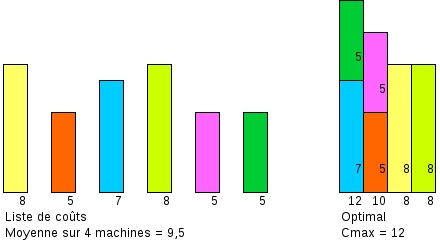
\includegraphics[width=\columnwidth]{MoyenneVsOptimal.jpg}
\caption{Liste de coût de départ, moyenne des tailles des jobs pour 4 machines, et makespan optimal.}
\label{ex:borneMinVSOptimalListeDepart}
\par}
\end{figure}

\begin{example}
Soit $P=\{8, 5, 7, 8, 5, 5\}$, l'ensemble des $p_i$ à appliquer sur 4 machines parallèles identiques:
La borne minimale $borne_{min} = \max \{ \max_i\{p_i\}, \frac{1}{m} \sum_{i=1}^{n} p_i \} = 9.5$ 
L'optimal $C_4^\star(J) = 12$ (figure \ref{ex:borneMinVSOptimalListeDepart}).
\end{example}

Cette borne minimale est égale à l'optimal uniquement si toutes les charges des machines sont identiques.
A partir d'une liste de coûts (synthétique ou naturelle) il est donc possible d'obtenir une instance dont l'optimal est connu. Cette opération nécessite la transformation de la liste de coût de départ pour un 
  nombre de machines défini (figure \ref{ex:maitriseOptimal}).
\begin{itemize}
	\item Soit une liste de $n$ jobs et l'ensemble des $p_i$ à appliquer sur $m$ machines parallèles identiques.
	\item Ordonnancement : Chaque job est affecté à la machine la moins chargée à ce moment là. 
	\item Tri : Tri des machines par ordre décroissant des charges.
	\item Complétion : La machine la plus chargée (la première) représente le MakeSpan. 
	      La charge des $m-1$ machines restantes est complétée pour obtenir le même temps d'exécution que la machine la plus 	          chargée .
	\item toutes les machines ont le même temps d'exécution. L'optimal, est dans ce cas égal à la 
	      moyenne des temps par machine. 
	      La nouvelle liste de coûts contient désormais $n + m-1$ éléments.
\end{itemize}

\bigskip 
Il convient de distinguer la liste de coût obtenue soit par génération, soit par récupération, 
  Native, dont seule la borne minimale est connue, 
  et sa transformée, complétée avec $m-1$ temps de jobs, nommée M1 (qui est une instance), 
  dont l'optimal est connu.
Tous les tests sont effectués sur les instances M1, et sur le nombre réel de tâches ($n + (m-1)$).

\begin{figure}
{\centering
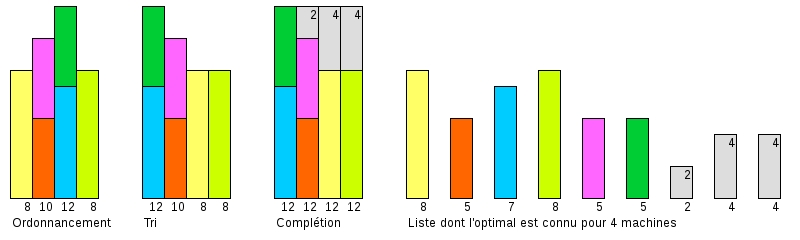
\includegraphics[width=\columnwidth]{maitriseOptimal.jpg}
\caption{transformation d'une liste pour obtenir l'optimal.}
\label{ex:maitriseOptimal}
\par}
\end{figure}

\subsection{indicateurs statistiques et caratéristiques}\label{ssec:instancesIndicateursStatistiquesCaratéristiques}

Afin de caractériser une liste de coût, plusieurs indicateurs statistiques sont calculés à la génération, ou à la récupération de celle-ci.
les calculs sont effectués via les bibliothèques ``scipy.stats'' (pour les moyennes géométrique 
  et harmoniques) et ``statistics'' de PYTHON.

Sont calculées et récupérées dans un champs tuple (évolutif) :
\begin{itemize}
	\item La moyenne de la charge par machine;
	\item La moyenne des éléments de $P$ (statistics.mean);
	\item La moyenne géométrique des éléments de $P$ ( scipy.stats.gmean );
	\item La moyenne harmonique des éléments de $P$ ( scipy.stats.hmean );
	\item La médiane de l'ensemble $P$ (stat.median);
	\item Le plus petit élément de $P$;
	\item Le plus grand élément de $P$;
	\item L'écart type des valeurs de $P$ (statistics.pstdev(l,statistics.mean(l)));
	\item La variance des valeurs de $P$  (statistics.pvariance(l, statistics.mean(l))).
\end{itemize}

Ces divers indicateurs peuvent donner une appréciation quant à 
  l'hétérogénéité d'une liste de coût.

\subsection{Conclusion}\label{ssec:instancesConclusion}

Nous venons de voir comment les listes de coûts sont générées et utilisées. 
Elles peuvent être créées via la production de nombres pseudo-aléatoires selon un nombre 
  défini de jobs et une distribution statistique choisie, 
  ou récupérées d'une archive de fichiers journaux de tâches relatifs à de réelles 
  activités de production.
De ces listes, peuvent être calculées des instances (M1) dont l'optimal est connu, 
  ce qui va permettre une estimation de l'efficacité des algorithmes.
Et enfin, plusieurs indicateurs statistiques caractérisant chaque instance les accompagnent.

Nous abordons maintenant la notion de ``campagnes'' de tests où les instances sont soumises à des heuristiques.  
   

\section{Campagnes}\label{sec:Campagnes}



\subsection{Implémentation des algorithmes}
\label{ssec:ImplémentationAlgorithmes}
Tous les algorithmes (étudiés) sont implémentés dans algorithms.py. Les procédures, objets et méthodes directement liés à ceux-ci sont placés dans ScheduleManagment.py i.e ceux qui n'ont pas le même prototype (FFD().). 
Ces algorithmes sont structurés sur le même principe :
\begin{itemize}

\item Les paramètres en entrée :
	\begin{description}

	\item Une liste de coûts : soit l'ensemble des $p_i$. 
	sous la forme $[p_1, p_2, ... , p_n]$. 
	Cette liste n'est pas forcément triée car cela fait partie 
	de l'heuristique, et ce tri peut changer d'une stratégie à l'autre.
	
	\item un nombre de machines m.
	\end{description}

\item Mesure du temps d'exécution. L'heure de début, et l'heure de fin 
sont consignées dans des variables ``before'' et ``after''. 
le temps d'exécution est donc mesuré en minutes-secondes.

\item Calcul du temps théorique, en fonction de la complexité théorique 
en temps de l’algorithme, ainsi que de la taille de la liste des temps, 
et du nombre de machines.

\item Déroulement de l'heuristique.

\item Retour d'un object ``PSched'' contenant les informations suivantes :
	\begin{description}
	\item Le nom de l'algorithme.
	\item Le temps attendu.
	\item le Makespan calculé
	\item Le temps qui a été nécessaire
	\item L'ordonnancement, sous forme de liste.
	\end{description}
\end{itemize}

\subsection{COMBINE}\label{ssec:COMBINE}

les problèmes de COMBINE 
l'algo approximatif (Do while et do until a son importance
Cu - Cl >= alpha A pas forcément ...
Condition d'arrêt n'integre pas le nombre de bin utilisées

\fco {Discuter avec Laurent/Louis-Claude/Julien de ce bug-si connu ou viens de moi}
!!! La borne supérieure  est donnée par LPT rule !!!
puis FFD est exécuté avec, c= borne supérieure + borne inférieure)/2. Or, si FFD est moins performant que LPT, le nombre de bin ne sera jamais égal au nombre de machines considéré. e.g si LPT( [p1,p2,...,pn]) sur m machines donne U, et FFD(U) donne V (avec V > U) FFD entre U et L (L<U) donnera au mieux V.....

COMBINE avec borne sup = 1.1Cmax(LPT), c'est ok

Corrections apportées
algorithme COMBINE
algorithme FFD

\subsection{fonctions annexes}\label{ssec:fonctionsAnnexes}

Quelques mots sur les fonctions appelées par les algorithmes principaux et qui ont leurs importance.

\begin{itemize}
\item FFD \cite{rieck2010basic} (implémentation)
\item Partitions LDM
\end{itemize}

\subsection{Ajout d'un algorithme}\label{ssec:AjoutAlgorithme}
Les sources sont disponibles, et l'application est prévue pour accueillir de nouveaux algorithme, si les règles suivantes sont respectées.

exemple avec MULTIFIT



\subsection{Génération d'une campagne}\label{ssec:generationCampagne}
Par choix de paramètres
Par exécution pré remplie
Par lecture d'une campagnes

\subsection{Gestion des "seeds"}\label{ssec:gestionSeeds}
si doit reproduire les mêmes instances


\subsection{Structure du fichier résultat}\label{ssec:StructureFichierResultat}

passage en revue des colonnes de leur provenance


\section{Comparaison des résultats} \label{sec:comparaisonResultats}

Comparer des algo quand on ne connaît pas l'optimal
par rapport au meilleurs résultat

\subsection{Normalisation du MakeSpan}
\label{ssec:normalisationMakeSpan}

trouver la bonne normalisation qui ne biaise pas trop la comparaison.
Mackespan sous forme brute, voire normalisé avec Cmax-optiml donne une courbe  accidentée et pas très lisible

\fco {Discuter avec Laurent/Louis-Claude/Julien si comparaison par graphes, ou voir moindres carrés ou autre méthode}

\begin{itemize}
\item MakeSpan brut
\item MakeSpan - optimal ou meilleur résultat
\item MakeSpan / optimal ou meilleur résultat
\item MakeSpan / Moyenne de tâche par machine
\end{itemize}

\subsection{Temps d'exécution} \label{ssec:tempsExécution}

 Le temps attendu est théorique et non absolu. i.e n log n ne donne pas un temps en minutes secondes.Le temps mesuré lui est donné en minutes secondes --> faire le lien entre estimation théorique et mesuré.
 
D'un algo a l'autre , Python est un langatge de haut niveau, donc pas évident. ce qui peut être comparé, c'est pour un même algo et faire varier N et/ou m. on compare les mêmes instructions....

faire un lien entre le théorique de une valeur pour comparer par la suite les résultats suivants
 
\subsection{Graphes}\label{ssec:graphes}
\fco {Discuter avec Laurent/Louis-Claude/Julien Libre et proposition de graphes, ou conduit}

Différents graphe à disposition
utilisation de ggplot
Modifier l'un d'eux
Abscisse 	= soit n
			= soit m
Couleurs = algorithme
pictogramme = méthode de génération instance (lambda, beta uniforme ...) 
taille = hétérogénéité ?? écart type ?? de l'instance




\section{Résultats} \label{sec:resultats}

\subsection{en fonction de n}\label{ssec:en fonction de n}

\subsection{en fonction de m}\label{ssec:en fonction de m}

\subsection{en fonction de n et m}\label{ssec:en fonction de n et m}

\subsection{en fonction des distributions et hétérogénéité}
\label{ssec:en fonction des distributions et hétérogénéité}



\section{P vers Q et R} \label{sec:P vers Q et R}

je ne sais pas encore

\section{Discussion} \label{sec:discussion}


\section{Conclusion} \label{sec:conclusion}

\begin{appendices}

\chapter{Génération des listes de nombres pseudo-aléatoires}

% \subsection{Objectifs}\label{ssec:synoptiqueObjectifs}

L'application doit permettre de reproduire un environnement expérimental d'exécution d'algorithmes liés au problème \problemGrahamP, et de les comparer entre eux au niveau de l'efficacité (borne d'approximation), et du coût en temps.
pour cela, il faut pouvoir :
\begin{itemize}
\item Générer des listes de temps de jobs selon différentes distributions et lois de probabilités, 
  afin de créer des instances (listes de temps de jobs~$+$~nombre de machines $m$) synthétiques. 
\item Récupérer des listes de temps existantes de chantiers réels disponibles au téléchargement, 
  permettant de créer des instances naturelles.
\item Caractériser ces listes de coûts de jobs, et ainsi estimer un niveau d’hétérogénéité 
  pour la mettre en relation avec le comportement des heuristiques.
\item Exécuter des heuristiques, récupérer leurs résultats (ordonnancement, Makespan) 
  et leur temps d’exécution 
  en fonction d'une liste de temps, et d'un nombre de machines $m$.
\item Exporter le résultats de plusieurs heuristiques soumises à 
  un environnement choisi 
  (instance, type  d'instance, variation du nombre de temps de jobs $n$, 
  variation du nombre de machines identiques $m$, algorithme utilisé) 
  dans le but de le soumettre à des scripts de statistiques et de comparaison (tableaux, graphes).
\item Archiver les différents résultats sous forme de données brutes, pour une utilisation future. 
\end{itemize} 
Pour finir, l'application se veut évolutive, et facilite, l'ajout d'heuristiques et de méthodes de générations de listes de temps.

% \subsection{Technologies utilisées}\label{ssec:synoptiqueTechnologiesUtilisées}

la partie applicative (génération d'instance, caractérisation des listes de temps, 
  exécution des algorithmes) est développée en PYTHON, et 
  la partie statistiques en langage R. 
Entre ces deux parties, les données brutes transitent via un fichier résultat au format CSV, 
 généré par le module PANDAS de PYTHON.
 
PYTHON et R ont été choisis pour les raisons suivantes :
\begin{itemize}
\item Temps de développement : ces langages, de haut niveau, permettent de développer 
  des solutions rapidement, avec une taille de code réduite.
\item Temps d'apprentissage : 
\item Se sont des langages interprètes : le fait que ces langages ne sont pas compilés 
  comprend plusieurs avantages. 
  D'une part, cela les rend (presque) indépendants des plate-formes d'exécution
  (la seule difficulté rencontrée, est l'adaptation à prévoir demeure dans la gestion des 
  chemins d'accès différente d'un OS à l'autre).
  D'autre part, les sources étant disponibles, cela permet une évolutivité de l’application. 
\item Les deux langages proposent des outils très efficaces permettant de travailler les listes.  
\item Abondances de bibliothèque : Il existe une multitude de bibliothèques permettant de 
  développer plus rapidement, 
  des fonctionnalités dans des domaines particuliers (mathématiques, statistiques, graphes, 
  structuration des données).

  e.g : 
  
  Pour PYTHON l'application utilise les bibliothèques 
  PANDAS (pour l'export des données data frame au format CSV) et 
  URLLIB (pour accéder au site de téléchargement et télécharger des listes de jobs existantes).

  Pour R, les scripts utilisent  
  READR (pour lire des fichiers CSV),  
  GGPLOT et PLOT3D (pour générer des graphes et les exporter au format PDF et JPG).
\item Ces plate-formes de développement sont gratuites. Ces langages sont donc largement utilisés 
  et la communauté est très active et productive,
  tant dans les tutoriels, 
  que dans les forums de discutions.         
\end{itemize}




\bigskip
Pour créer des listes de coûts, nous utilisons la bibliothèque par défaut de génération de 
  nombres pseudo-aléatoires de PYTHON, selon différentes règles statistiques. 
Ceci permet de créer des listes, pourvues de diverses propriétés, notamment l’hétérogénéité. 

\bigskip
Les deux types de générations suivants, implémentés dans l'application, 
  génèrent des nombres entiers \footnote{\samepage La commande random.uniform(a,b) de PYTHON renvoie un réel. L'application le transforme en entier, à l'aide de la commande round(n).}, mais ne permettent pas la maîtrise de la variance. 
Ce sont les deux seuls types de génération utilisés dans le protocole expérimental de comparaisons des heuristiques dans \cite{della2020longest}.
   
\begin{itemize}
\item Uniforme : les nombres pseudo-aléatoires générés, sont uniformément répartis 
  entre deux entiers $a$ et $b$.
   
  \begin{lstlisting}[language=Python]
	for i in range(n):
		rand = random.uniform(a,b)
  \end{lstlisting}

\item Non-uniforme. définie en tant que ``NON-UNIF'' dans \cite{frangioni2000multi}. Cette méthode produit 
  une liste de temps de traitements dont 
  $98\%$ des éléments sont uniformément répartis dans l’intervalle  $[0.9 (b-a), b]$, et 
  le reste ($2\%$) est uniformément réparti dans l'intervalle  $[a, 0.2 (b-a)]$.


  \begin{lstlisting}[language=Python]
	n98 = int((98*n) / 100)
	    a1 = 0.9*(b-a)
    	b1 = b
    	a2 = a
    	b2 = 0.2*(b-a)
		...
    	for i in range(n98):
       		rand = random.uniform(a1,b1)

    	...
    
    	for i in range(n-n98):
    		rand = random.uniform(a2,b2)
  \end{lstlisting}
  
\end{itemize}

\bigskip
L'application implémente d'autres type de générations, basés sur des lois statistiques (distribution). 
Celles-ci génèrent des nombres réels, et acceptent des paramètres qui ont un effet sur 
  ``l'écrasement'' des courbes représentant les distributions, 
  et entrent dans le calculs de la variance.

\begin{itemize}
\item Loi gamma : La loi gamma représente généralement des manifestions qui se déroulent dans le temps. Elle accepte deux paramètres $k$ (``alpha'' dans l'implémentation) qui affecte la forme, et $\Theta$ (``beta'' dans l’implémentation) qui affecte l'échelle.  
  \begin{lstlisting}[language=Python]
	for i in range(n):
    		rand = random.gammavariate(alpha,beta)
  \end{lstlisting}
\item Loi exponentielle : Cas particulier de la loi gamma. Elle représente la durée de vie d'un événement. Elle accepte un paramètre $\lambda$ (lambda dans l'implémentation) qui affecte l'échelle.  
  \begin{lstlisting}[language=Python]
	for i in range(n):
    		rand = random.expovariate(lambd)
  \end{lstlisting}

\item Loi beta. Accepte deux paramètres de forme (un pour l'implémentation), $\alpha$ (alpha dans l’implémentation) qui affecte la forme, et $\beta$ (toujours à 1 dans l'implémentation) qui affecte aussi la forme.
  \begin{lstlisting}[language=Python]
	for i in range(n):
    		rand = random.betavariate(alpha,1)
  \end{lstlisting}

\end{itemize}

\bigskip
\paragraph{Seed} Chaque génération d'instance est accompagnée de la récupération d'une graine (seed). 
Chaque instance a sa propre graine, et est stockée aussi dans le fichier de résultats. 
Ainsi il est aisé de reproduire à l'identique une liste de coûts, en utilisant la même graine 
  lors de sa ré-génération. 
 





\end{appendices} 



\bibliographystyle{plain}				% NE PAS ENLEVER !!!!!!!!!!
\bibliography{Bibliographie}			% Utilise Bibliographie.bib


\end{document}
